
\chapter[Intégration à l'environnement industriel]{Intégration à l'environnement industriel}

\boitemagique{Dans ce chapitre}{
Ce chapitre présente les liens entre explicabilité et problématiques de Pôle emploi. Nous décrivons le cadre logiciel \textit{Gabarit} et les développements de la thèse réalisés dans ce dernier. Les apports de la démarche d'explicabilité aux  engagements éthiques sont présentés. Enfin, nous proposons un guide des méthodes d'explicabilité dédiées à l'industrie.
}

% intro
Ce chapitre présente l'intégration des travaux de cette thèse dans l'environnement industriel de Pôle emploi.
% Quoi
Les liens entre ces travaux et l'entreprise sont multiples. D’un point de vue technique les contributions d’explicabilité présentées sont implémentées dans l'infrastructure de développement de Pôle emploi : \textit{Gabarit}. %outil open source destiné à la mise en production de modèles d'apprentissage automatique.
D’un point de vue des enjeux éthiques autour de l'IA chez Pôle emploi, ce chapitre participe à la mise en place et à la réponse aux exigences de la charte éthique IA.

% Objectif du chapitre
Nous présentons l'apport cette thèse à l'outil, en section~\ref{C6:gabarit}. La section~\ref{C6:ethique}, montre la contribution de la thèse pour la mise en œuvre de la charte éthique Pôle emploi. Enfin, un guide est proposé en section~\ref{C6:guide} afin de choisir d'une méthode d'explicabilité dans un contexte industriel.

\section{Gabarit} \label{C6:gabarit}

% intro
Dans cette section, nous présentons \textit{Gabarit}\footnote{\url{https://github.com/OSS-Pole-Emploi/gabarit}}, un outil open source créé par Pôle Emploi. Sous la forme de module python, il permet de générer des projets d'apprentissage automatique prêts à l'emploi.
% Pourquoi
Il permet ainsi d'uniformiser les pratiques, favoriser le partage, accélérer la mise en production des modèles d'IA.
% Objectif du chapitre
Dans ce chapitre, nous présentons l'historique de l'outil, sa philosophie, et comment s'y intègrent mes travaux de thèse.

\subsection{Historique} \label{C6:historique}

% participation active mais avant la thèse
Les premiers travaux de création d'outillage communs autour de la donnée démarrent en 2018. Ils sont liés au besoin du département \textit{Agence Data Services} d'unifier les processus spécifiques de nettoyage de données textuelles. Cet outil, nommé \textit{Words'n'fun}, présente un ensemble de fonctions python pour le prétraitement de textes\footnote{\url{https://github.com/OSS-Pole-Emploi/words_n_fun}}.
% participation active mais avant la thèse
Ce besoin d'uniformisation des bonnes pratiques s'étend au développement de modèles d'IA en NLP. La volonté est de faciliter leur mise en production et le transfert du projet d'une personne à l'autre. Le \textit{Template NLP} est créé en 2019, en tant que projet git à télécharger. Il est axé sur l'entraînement, la sérialisation et la mise à disposition de modèles d'IA. L'outil est un générateur de projets, il embarque et intègre divers outils open source pour
historiser les données avec \textit{Data Version Control} (DVC)\footnote{\url{https://dvc.org/}} et les prétraiter avec \textit{Words'n'fun}),
effectuer l'apprentissage automatique (\textit{Scikit-Learn}\footnote{\url{https://scikit-learn.org/}}, \textit{Tensorflow}\footnote{\url{https://www.tensorflow.org/}}  et \textit{Torch}\footnote{\url{https://pytorch.org/}}),
aider au suivi des modèles (\textit{MLflow}\footnote{\url{https://mlflow.org/}}, \textit{Artifactory}\footnote{\url{https://jfrog.com/fr/artifactory/}})
ainsi qu'un démonstrateur \textit{Streamlit}\footnote{\url{https://streamlit.io/}}.

Pour faciliter sa prise en main par les scientifiques des données de l'entreprise, une formation au travers de tutoriels interactifs est mise en place. Les travaux de cette thèse sont réalisés en utilisant cet outil, contribuant ainsi directement à l'ajout de fonctionnalités d'explicabilité.

En 2020 et 2021 sont intégrés au \textit{Template NLP} les \textit{Template vision} et \textit{Template numérique}, gérant respectivement les données tabulaires et les images. L'outil évolue selon les besoins et les contraintes de mise en production.
Dès le démarrage du projet, son ouverture à la communauté open source est considérée. En 2022, le service juridique donne son aval pour que le code soit rendu disponible sous licence copyleft; ce qui donne lieu à des travaux de refonte. Un des points principaux est la traduction en anglais, car le code interne Pôle emploi est historiquement écrit en anglais avec des commentaires français, ce qui limite le partage à la communauté. Les tests sont améliorés pour consolider le projet, et l'installation est facilitée en partageant le projet sous forme de module python. Le tout est rendu public en 2022 sous le nom \textit{Gabarit}.

% D'abord le template NLP avec la gestion sklearn/tensorflow (torch par la suite) et intégration dvc/mlflow/words\_n\_fun; gestion des embeddings, des différents datasets etc...
% Ensuite on a rajouté le template vision (en avance de phase) pour tout ce qui est CV, puis le template numerique pour les données tabulaires plus classiques

L'outil \textit{Gabarit} est composé de 2 éléments : le générateur de projets et le projet généré à utiliser. Le générateur est présenté dans la section suivante, et le projet généré est présenté à la suite.

\subsection{Le générateur de projets}

Le générateur de projets permet de créer un projet d'IA en une ligne de commandes. Il gère notamment les formats de données lus et sérialisés (encodage, séparateur de colonne des fichiers csv...), et les éventuels outils à configurer tel que DVC.

Une fois le module installé (ou mis à jour), il est directement possible de créer un nouveau projet. La ligne de commande permet de générer un projet d'analyse de textes (\textit{generate\_nlp\_project}), d'images (\textit{generate\_vision\_project}) ou de données tabulaires (\textit{generate\_num\_project}).
D'autres précisions optionnelles sont disponibles pour la gestion du projet : intégration de DVC, configuration spécifique (encodage...), etc. Plus de détails sont donnés dans la documentation du projet.

Le générateur repose sur une arborescence de fichiers ``templates'' correspondant chacun à une typologie de données (texte, image et tabulaire). Chaque \textit{template} contient le code source presque prêt à l'emploi : il ne reste qu'à remplacer le nom du projet, à la manière d'un texte à compléter, ce qui est effectué automatiquement lors de la génération du projet.
% En complément, de l'arborescence de fichiers ainsi complétée qui va constituer le cœur du projet IA, celui-ci va également comporter de nombreuses suites de tests permettant de valider le bon fonctionnement des fonctionnalités proposées ainsi que des jeux de données jouets permettant de faciliter la prise en main du code généré au travers d'un tutoriel.
Le générateur peut ainsi créer le projet souhaité avec le nom et l'emplacement donnés, ainsi que les spécifications optionnelles. Tous les fichiers sont générés pour être prêts à l'emploi.

\subsection{Architecture du projet généré}

Une fois le projet généré et installé, tout le code du projet peut être modifié par le scientifique des données qui y a un accès direct, à la différence d'outils plus graphiques tels que Dataiku. Il reste possible d'intégrer par la suite tout module python souhaité. C'est également le moment idéal pour démarrer l'historisation sur \textit{git}, si cela n'a pas déjà été mis en place.

Une fois le projet installé, il ne reste plus qu'à intégrer les données souhaitées. Des fonctions sont à disposition pour prétraiter les données. Des architectures de modèles d'apprentissage automatique sont à disposition des utilisateurs,  basées sur le trio \textit{Scikit-learn}, \textit{Tensorflow}, \textit{Pytorch}.
Il est possible d'entraîner directement un de ces modèles, d'ajuster leur architecture, ou encore d'en créer un nouveau, le tout avec très peu de modifications de code à effectuer. Les architectures de modèle couvrent à la fois l'apprentissage automatique et profond.

La figure~\ref{fig:api_gabarit} illustre les six fonctionnalités liées directement au modèle et à son cycle de vie, à savoir : le définir, l'entraîner (méthode \textit{fit}), l'enregistrer et recharger (\textit{save} et \textit{load\_model}), l'utiliser pour prédire un résultat (\textit{predict}) et expliquer celui-ci (\textit{explain}).
\begin{figure}[htpb!]
\centering
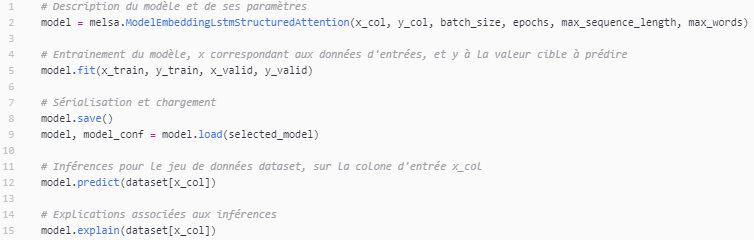
\includegraphics[width=\textwidth]{S5-Presentation_du_template_nlp/figures/usage_gabarit.png}
\caption{Illustration des fonctionnalités de \textit{Gabarit} pour un modèle : définition, entraînement, sérialisation, chargement, inférence et explication.}
\label{fig:api_gabarit}
\end{figure}

L'architecture de chaque modèle est disponible dans un script associé, ce qui permet notamment d'ajouter, supprimer, modifier des couches de réseaux.

Le projet intègre également des interfaces avec divers outils, notamment un démonstrateur via une page web, et la mise à disposition du modèle via \textit{artifactory} afin d'être utilisé dans différents services et outils.

Cet environnement a servi de base pour les développements des travaux présentés ici. De même, les travaux ont nourri l'outil \textit{Gabarit}. Nous présentons cet échange dans la section suivante.

\subsection{Intégration des travaux d'explicabilité}

Les travaux présentés ici sur l'explicabilité des algorithmes ont été développés dans \textit{Gabarit}. Le modèle à attention présenté en chapitre 4 a été conçu au sein de l'outil, ainsi que les développements liés aux explications globales. De même, le démonstrateur fourni a servi de base aux illustrations des différentes méthodes d'explications.

Réciproquement, une partie des avancées de cette thèse ont servi à enrichir l'outil. Le principal avantage est l'intégration directe d'une méthode d'explicabilité pour tout modèle, via la méthode \textit{model.explain}. L'explication est par défaut apportée par Lime~\cite{Ribeiro2016}, une méthode agnostique au modèle parmi les plus légères, et en moyenne plus rapide que les ancres utilisées dans les chapitres 3 et 4. Lime sert de premier point de référence pour les scientifiques des données. Notre état de l'art montre qu'il existe toutefois d'autres méthodes intéressantes.

L'architecture du modèle à attention utilisé y est mise à disposition en générant un projet d'analyse de textes, via la classe \textit{ModelEmbeddingLstmStructuredAttention}. Les explications par attention sont récupérables, à titre expérimental et pour cette classe uniquement, via la méthode \textit{model.explain\_indexes}. %À noter que cette partie de l'outil n'est pas passée par les mêmes tests rigoureux d'industrialisation que les autres modèles et méthodes.
L'intégration au fil de l'eau des contributions au cadre logiciel permet aux équipes de Pôle emploi ou autres utilisateurs de l'outil d'intégrer la notion d'explicabilité à tous les modèles d'IA.

Pour conclure brièvement sur cette section, \textit{Gabarit}, a accéléré la mise à disposition des développements effectués dans le cadre de cette thèse. En l'employant, nous avons facilité l'accès aux travaux d'explicabilité, pour les équipes de Pôle emploi, mais également à toute personne intéressée.

L'outil étant conçu pour faciliter la mise en production d'outils d'IA, il possède toutefois des contraintes non adaptées à un environnement de recherche pure. C'est un outil lourd, faisant appel à de nombreuses dépendances. Celles-ci sont ajustables grâce à la modification directe du code python, mais il est contre-productif de s'écarter totalement du cadre prévu. Ainsi, les premiers développements de cette thèse se sont faits avant l'intégration de Pytorch, ce qui a contraint à réaliser les développements sur tensorflow.

Les travaux mentionnés dans cette section ont été techniques, mais ce n'est pas le seul apport pour l'entreprise. La section suivante montre leur intérêt dans la réflexion éthique réalisée à Pôle emploi.

\section{\'Ethique} \label{C6:ethique}

L'éthique de l'IA est un enjeu présent à Pole emploi depuis 2018. La figure~\ref{fig:chronologie_ethique}  montre la chronologie et les grands points d'étape de la réflexion autour de ces enjeux. Les étapes auxquelles j'ai activement contribué, notamment en participant aux réunions d'avancement, sont encadrées en noir. L'éthique est d'abord abordée par le prisme de la maitrise des risques. Les premiers travaux mènent à la construction de la \textit{charte pour une IA éthique}~\cite{Pole2022}. C'est en parallèle et dans le même contexte que les travaux de la présente thèse sur l'explicabilité des algorithmes d'IA sont proposés, le sujet étant affiné au long de l'année 2019.
% 17% de la population de 15+ ans en situation d'illectronisme, enquête menée dans les Hauts de France en 2019, Insee, enquête TIC ménages 2019, RP 2016.

\begin{figure}[htpb!] % TODO trait + gros
\centering
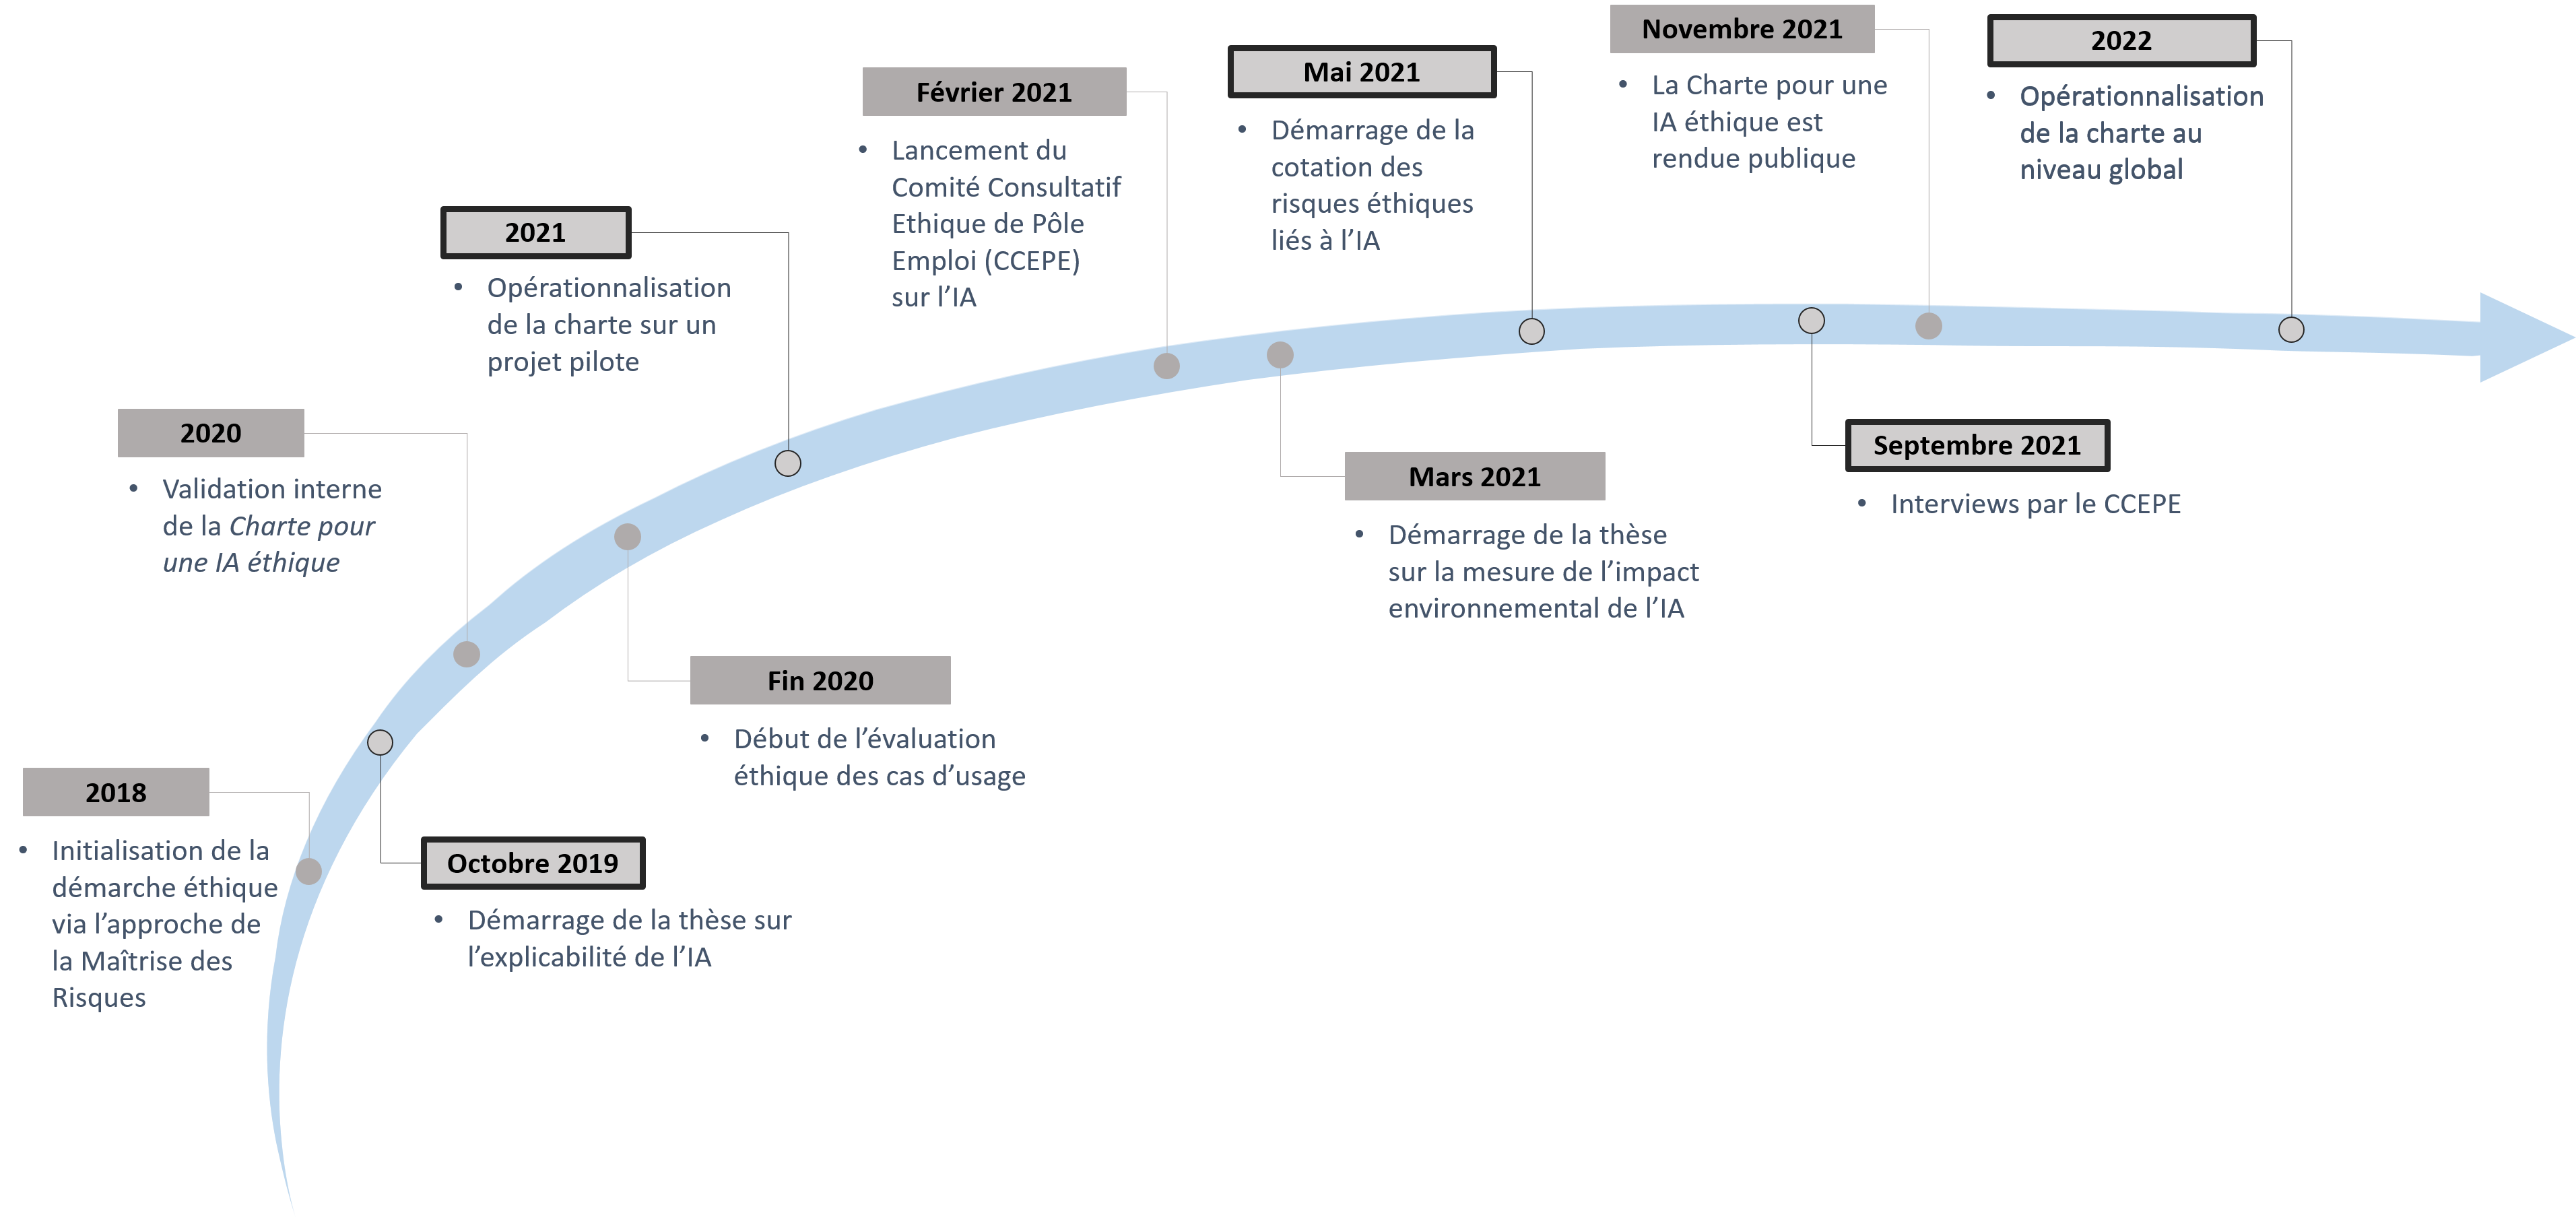
\includegraphics[width=\textwidth]{S5-Presentation_du_template_nlp/figures/ethique_chrono.png}
\caption{ Chrolonogie des projets et évènements liés à l'éthique à Pôle Emploi depuis 2018. Les projets encadrés en noir sont ceux auxquels j'ai activement participé.}
\label{fig:chronologie_ethique}
\end{figure}

Ainsi, avec les réflexions entamées en 2018, la \textit{charte pour une IA éthique} fait son apparition dès 2020. Un premier point d'évaluation de l'existant est alors effectué dans la foulée.
La figure~\ref{fig:chronologie_ethique} montre l'accélération des travaux en 2021.
Un projet pilote met en place une première salve d'ateliers d'\textit{opérationnalisation} de la charte.

En début d'année, la création du \textit{Comité Consultatif \'Ethique de Pôle Emploi} (CCEPE) est actée. Ce comité externe est composé de dix experts d'horizons complémentaires : universitaires, représentants de syndicats et des usagers. Ce CCEPE a pour vocation d'accompagner et porter un regard externe critique sur les engagements et actions de l'établissement. Dans ce cadre, le CCEPE a dialogué activement avec les acteurs de Pôle emploi, me permettant de présenter l'avancée des travaux sur explicabilité.

Par la suite, les travaux de thèse d'Angela Ciocan sur la mesure de l'impact environnemental de l'IA démarrent.
Les risques éthiques liés à l'IA sont évalués de façon plus globale pour tous les sujets existants et à venir. Les ateliers de cotation de ces risques mêlent des profils techniques et managériaux. Ces cotations sont une première étape permettant l'opérationnalisation de la charte.

Par la suite, nous présenterons la charte et ses grands principes en section~\ref{C6:charte}. Sa mise en œuvre est traitée, de la cotation des risques à la l'établissement d'outils pour les acteurs des projets IA, en section~\ref{C6:ope_charte}.

\subsection{La charte éthique} \label{C6:charte}

La charte est publiée en interne dans un premier temps, puis publiquement en Novembre 2021. Elle est donc disponible sur le site de communication officiel de Pôle emploi\footnote{\url{https://tinyurl.com/charteIA}}. Elle est également en annexe en section~\ref{A:charte_pe}.
Cette charte répond au besoin de suivi interne, mais également à la volonté d'être auditables.

Les 7 axes de la charte :
\begin{enumerate}
    \item Finalité et légitimité des algorithmes,
    % Inadéquation entre les finalités des algorithmes et solutions d'IA, et les missions de PE telles que décrites dans l’article L5312 du code du travail
    \item L’humain au centre ; l’intelligence artificielle au service de l’humain,
    % Absence de compréhension du sens et des enjeux du recours à l'IA dans les solutions : méfiance, non-utilisation des solutions, etc. (culture change)
    \item Equité et non-discrimination,
    % Défaillance ou absence de mesures permettant de garantir l’équité de traitement entre les utilisateurs
    \item Liberté de choix,
    % Absence de temps laissé aux agents et aux usagers pour la prise de décision
    \item Transparence,
    % Défaillance ou absence dans la capacité à expliquer le fonctionnement d'un algorithme et ses résultats (règles que se donne l'algorithme)
    % Défaillance ou absence d'explication détaillée et sous forme intelligible du résultat algorithmique par le responsable de traitement
    \item Sécurité,
    % Défaillance ou absence de la qualité de la collecte et du traitement des données
    \item Impact environnemental.
    %Absence de mise en place d'un indicateur multicritère d’impact en collaboration avec l’INR
\end{enumerate}
% + risques associés ajoutés

% Plus éloigné ; en parler un peu
\paragraph{Finalité et légitimité des algorithmes}
Cet axe implique d'utiliser les outils d'IA à bon escient, dans le but de fournir un service bénéfique ou de lutter contre les actes de malveillance.

\paragraph{L’humain au centre ; l’intelligence artificielle au service de l’humain}
Les outils sont créés pour accompagner l'humain dans ses tâches habituelles. Pôle emploi indique dans sa charte s'engager à fournir ``une explication sur le fonctionnement d'un service ou une aide à la décision'' ainsi que ``des actions d'accompagnement et de sensibilisation [...] à l'intelligence artificielle'' aux utilisateurs internes (\textit{agents}) et externes (\textit{usagers})~\cite{Pole2022}.

\paragraph{Equité et non-discrimination}
Il s'agit ici à la fois de reconnaitre que l'IA peut ``reproduire, renforcer ou générer des biais discriminatoires'', et veiller à limiter l'impact de ceux-ci~\cite{Pole2022}. Le contexte applicatif de l'établissement est à risque du fait de biais humains présents dans le monde du travail. Les discriminations à l'embauche ou les métiers dits ``genrés'' en sont des exemples.

\paragraph{Liberté de choix}
Les décisions prises par un algorithme peuvent toujours être modifiées par un humain, et les utilisateurs ont accès à un interlocuteur pour demander un tel recours. Il est toujours possible d'ignorer les recommandations des algorithmes d'aide à la décision. En d'autres termes, l'humain a le dernier mot.

\paragraph{Transparence}
Cet axe répond aux exigences du RGPD et de la loi pour une république numérique~\cite{Legifrance2016}.
Il comprend le recueil du consentement éclairé des utilisateurs pour collecter et traiter leurs données.
La transparence concerne ici l'information aux utilisateurs lorsqu'iels ont à faire à un outil automatique, potentiellement basé sur l'IA. Cette exigence couvre notamment les agents conversationnels (ou ``chatbots'').
La charte indique très clairement que l'indication de l'utilisation d'un service d'IA s'accompagne de la ``capacité d'expliquer de la façon la plus compréhensible possible son fonctionnement et ses résultats''~\cite{Pole2022}.
% https://www.legifrance.gouv.fr/codes/article_lc/LEGIARTI000034195881 article R. 311-3-1-2 du Code des relations entre le public et l'administration
% https://www.legifrance.gouv.fr/codes/article_lc/LEGIARTI000033205535/  l'article L. 311-3 du Code des relations entre le public et l'administration

\paragraph{Sécurité}
La sécurisation concerne le traitement de données personnelles et sensibles, les paiements et la lutte contre les attaques (fraudes, arnaques, vol de données). Dans le cadre de l'IA, il s'agit notamment de valider l'usage de données personnelles et sensibles, si nécessaire les anonymiser. La sécurisation des services passe également par la vérification de leur résistance aux attaques adversaires. % TODO verif que attaques adversariales décrites avant, si oui crossref

\paragraph{Impact environnemental}
Dans une démarche d'usage responsable des outils à disposition, Pôle emploi reste attentif à l'impact et au coût environnemental des solutions développées. La démarche étant déjà entamée pour des développements hors IA, il s'agit ici d'une adaptation des bonnes pratiques existantes au développement, spécifique, des modèles d'apprentissage automatiques et profonds.

% Ici faire référence aux chapitres y afférent
Les travaux présentés dans ce manuscrit s'inscrivent directement dans deux des axes de la charte. Pour respecter les engagements des axes de \textit{l'humain au centre}, et de la \textit{Transparence}, il faut être en mesure d'expliquer le fonctionnement des algorithmes d'IA utilisés, dans leur fonctionnement global mais également lors de recours pour un résultat spécifique.


\subsection{Mise en œuvre de la charte} \label{C6:ope_charte}

La création de la charte est une première étape, mais son existence ne suffit pas à rendre les travaux entamés et révolus plus éthiques. Après une première étude sur un projet pilote, la mise en œuvre globale de la charte s'est faite en deux temps.

%  C:\Documents\Expertise XAI, Ethique\20201027_IE_Evaluation éthique_Mails_V1.6
Le projet pilote étudié porte sur l'analyse de mails afin d'assister les agents Pôle emploi. L'objectif est d'apposer une étiquette à chaque mail reçu par un conseiller : s'agit-t-il d'une demande de rendez-vous ? D'une réclamation ? Ces étiquettes permettent aux agents de s'organiser et construire leur planning plus facilement, en traitant ensemble toutes leurs demandes de rendez-vous, par exemple.  Ce projet pilote à l'avantage de faire appel à de nombreuses notions d'éthique (sécurité des données, non-discrimination, assistance et non remplacement du travail des conseillers...).
L'étude met en avant les caractéristiques spécifiques de ce projet avec ses acteurs, les données traitées etc. Les sept axes de la charte sont abordés un à un, et les points d'attention sont abordés avec les risques associés, les mesures déjà mises en place et les améliorations envisageables.

% 4. a) Ethique > 3 > carto
Les travaux de mise en œuvre de la Charte se sont par la suite généralisés à tous les cas d’usage IA de Pôle emploi.
La première étape a été la cotation des risques associés à chaque axe de la charte, selon leur probabilité et leur impact. Un risque est, par exemple une \textit{défaillance ou absence dans la capacité à expliquer le fonctionnement d'un algorithme et ses résultats (règles que se donne l'algorithme)}.
La probabilité d'occurrence $P$ de ce risque est quantifiée entre $1$, très peu probable, et $4$, fréquent. Les impacts sont également notés entre $1$ pour un impact faible, et $4$ pour un impact capital. Ces impacts sont évalués au travers de $6$ catégories:
\begin{enumerate}
    \item l' \textbf{image}, interne et médiatique, de l'établissement,
    \item les \textbf{finances} englobant les risques de pertes financières ou dépenses imprévues,
    \item \textbf{réglementaire}, allant du non-respect de la charte jusqu'au risque pénal,
    \item la réalisation des \textbf{missions}, comprenant les retards, la non réalisation des missions confiées,
    \item le \textbf{climat social} interne, comprenant les tensions pour les agents, allant jusqu'au risque de grève,
    \item l'\textbf{humain}, prenant en compte les agents et les usagers (demandeurs d'emploi et recruteurs).
\end{enumerate}
Ces impacts sont cotés collégialement grâce à un panel d'agents référents techniques, métiers, décisionnaires. La gravité $G$ du risque est calculée en fonction des cotations selon l'équation :
\begin{equation}
    G = P * \frac{I_{Image} + I_{Finance} + I_{Reglementaire} + I_{Mission} + I_{Social} + I_{Humain}}{6}
\end{equation}
Le risque est considéré peu grave lorsque $G \in [1, 4[$, et préoccupant lorsque $G \in [12,16]$.


À titre d'illustration, sans les travaux de cette thèse, la gravité de ce risque est de $4* (3+1+4+3+3+4)/6 = 12 $.
Avec la prise en compte de ces travaux, la gravité devient $ 1* (3+1+4+3+3+4)/6 = 3 $. Le risque, auparavant préoccupant, est alors peu grave. Cette illustration est tirée de la documentation interne de Pôle emploi, les chiffres sont à titre d'illustration seulement~\cite{Pole2021}.

La seconde étape de cotation consiste à déterminer les actions associées aux risques détectés, afin de diminuer l'impact de ceux-ci. Les actions peuvent diminuer les impacts ou la probabilité d'occurrence des risques. Ces actions sont globales, générales afin de s'adapter à tout projet. Reprenons le risque d'incapacité à expliquer un algorithme. Une action liée peut être \textit{Utiliser lorsque c'est possible des algorithmes et des solutions d'explicabilité afin d'être transparent sur les décisions prises}. Ces actions globales sont complétées par des précisions opérationnelles : tâches à mener, acteurs impliqués, moyens nécessaires et moment privilégié pour réaliser l'action. Dans l'exemple mentionné portant sur l'explicabilité, les travaux présentés dans ce manuscrit ont servi de base aux réflexions, apportant une vision des solutions existantes, et une preuve de première application.

%  s'établit en quatre phases synchronisées avec la vie du projet, comme le montre la figure
% \begin{figure}[htpb!]
% \centering
% 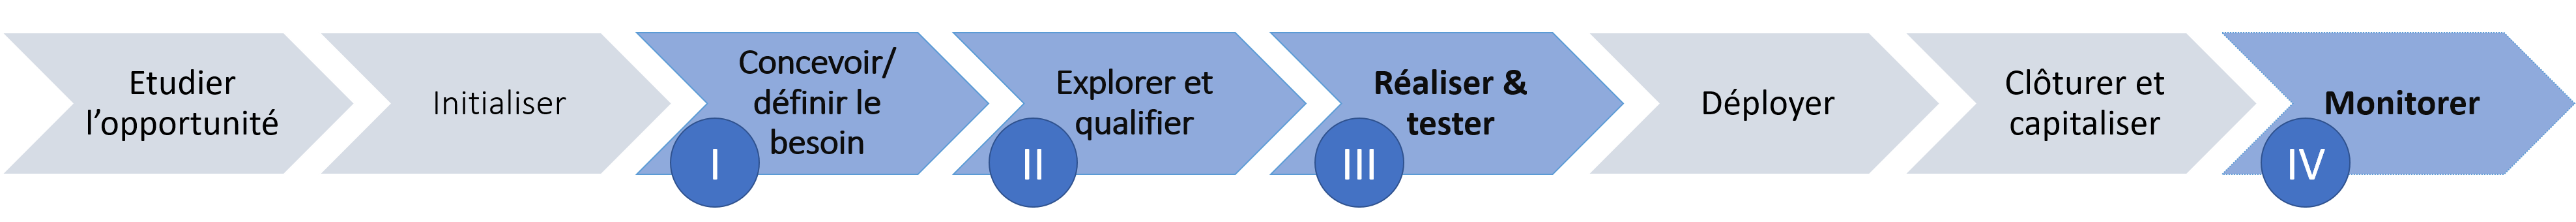
\includegraphics[width=\textwidth]{S5-Presentation_du_template_nlp/figures/phases_etude_ethique.png}
% \caption{Les quatre phases d’études}
% \label{fig:chronologie_ethique}
% \end{figure}

% Conclusion : avancées, limites
Les travaux sur l'éthique ainsi que la cartographie des risques présents ont bénéficié, pour deux des sept axes de la charte, des réflexions engagées ici. Nous avons montré que nous pouvons réduire les risques rencontrés, en passant d'une volonté d'explicabilité à une application concrète de méthodes d'explications sur nos données, présentés en chapitres 2 et 4. Ces avancées nécessitent toutefois une priorisation et un suivi adéquats par les personnes en charge des différents projets. Nous conclurons cette section en soulevant le questionnement suivant : le devoir d'expliquer un résultat ou le fonctionnement d'un service doit-il être exigé uniquement lorsque ce dernier est basé sur des algorithmes d'intelligence artificielle ?

De manière concrète, et issue des savoirs engrangés dans cette aventure de trois ans, nous proposons à cet effet un guide permettant de faire le tri parmi les nombreuses méthodes d'explicabilité, en fonction des objectifs à atteindre.

\section{Comment choisir une méthode d'explicabilité ?} \label{C6:guide}

Cette section présente un guide permettant de déterminer les caractéristiques souhaitées pour une méthode d'explication. Les éléments de la section~\ref{C1:typologie} sont repris et organisés afin d'aider à la détermination de caractéristiques idéales pour un projet donné, en fonction de ses contraintes. Ce guide est inspiré de travaux existants~\cite{Vermeire2021}, simplifié et adapté au contexte industriel.

% objectif
Cette section fournit ainsi des outils qui aideront le lecteur ou la lectrice à déterminer ses besoins, et \textit{in fine} à sélectionner un panel restreint de méthodes de la littérature qui conviendront le mieux à ces besoins.
% plan


\paragraph{Guide des caractéristiques recherchées}
% quoi
Pour déterminer les systèmes d'explication préférables dans un projet, il faut au préalable déterminer les caractéristiques recherchées.
% comment
Pour déterminer ces caractéristiques, il faut avoir en tête l'objectif, le public, et le contexte de réception des explications. Il est possible que pour un même modèle d'IA, plusieurs besoins d'explicabilité soient détectés, à des moments de vie différents.
Dans ce cas, l'exercice proposé dans cette section est à réaliser pour chaque besoin.

% objectifs
Cette section propose un guide, permettant de définir les caractéristiques souhaitées pour un système d'explication.
% plan
Chaque caractéristique vue en introduction est passée en revue, à savoir la portée, la stratégie, et le format d'explication.

\paragraph{Choix de la portée}
%facteurs dominants
Les données principales permettant de choisir la portée de l'explication sont les utilisateurs et leurs objectifs.
%rappel options
Tel que vu en introduction, une explication de portée globale permet de construire la confiance dans le modèle sur son comportement général. Elle est pertinente pour les phases de validation et d'appropriation du modèle.
Une explication locale permet de se concentrer sur un résultat, et est plus proche des conditions réelles de l'utilisation du modèle.

\begin{figure}[htpb!]
    \centering
    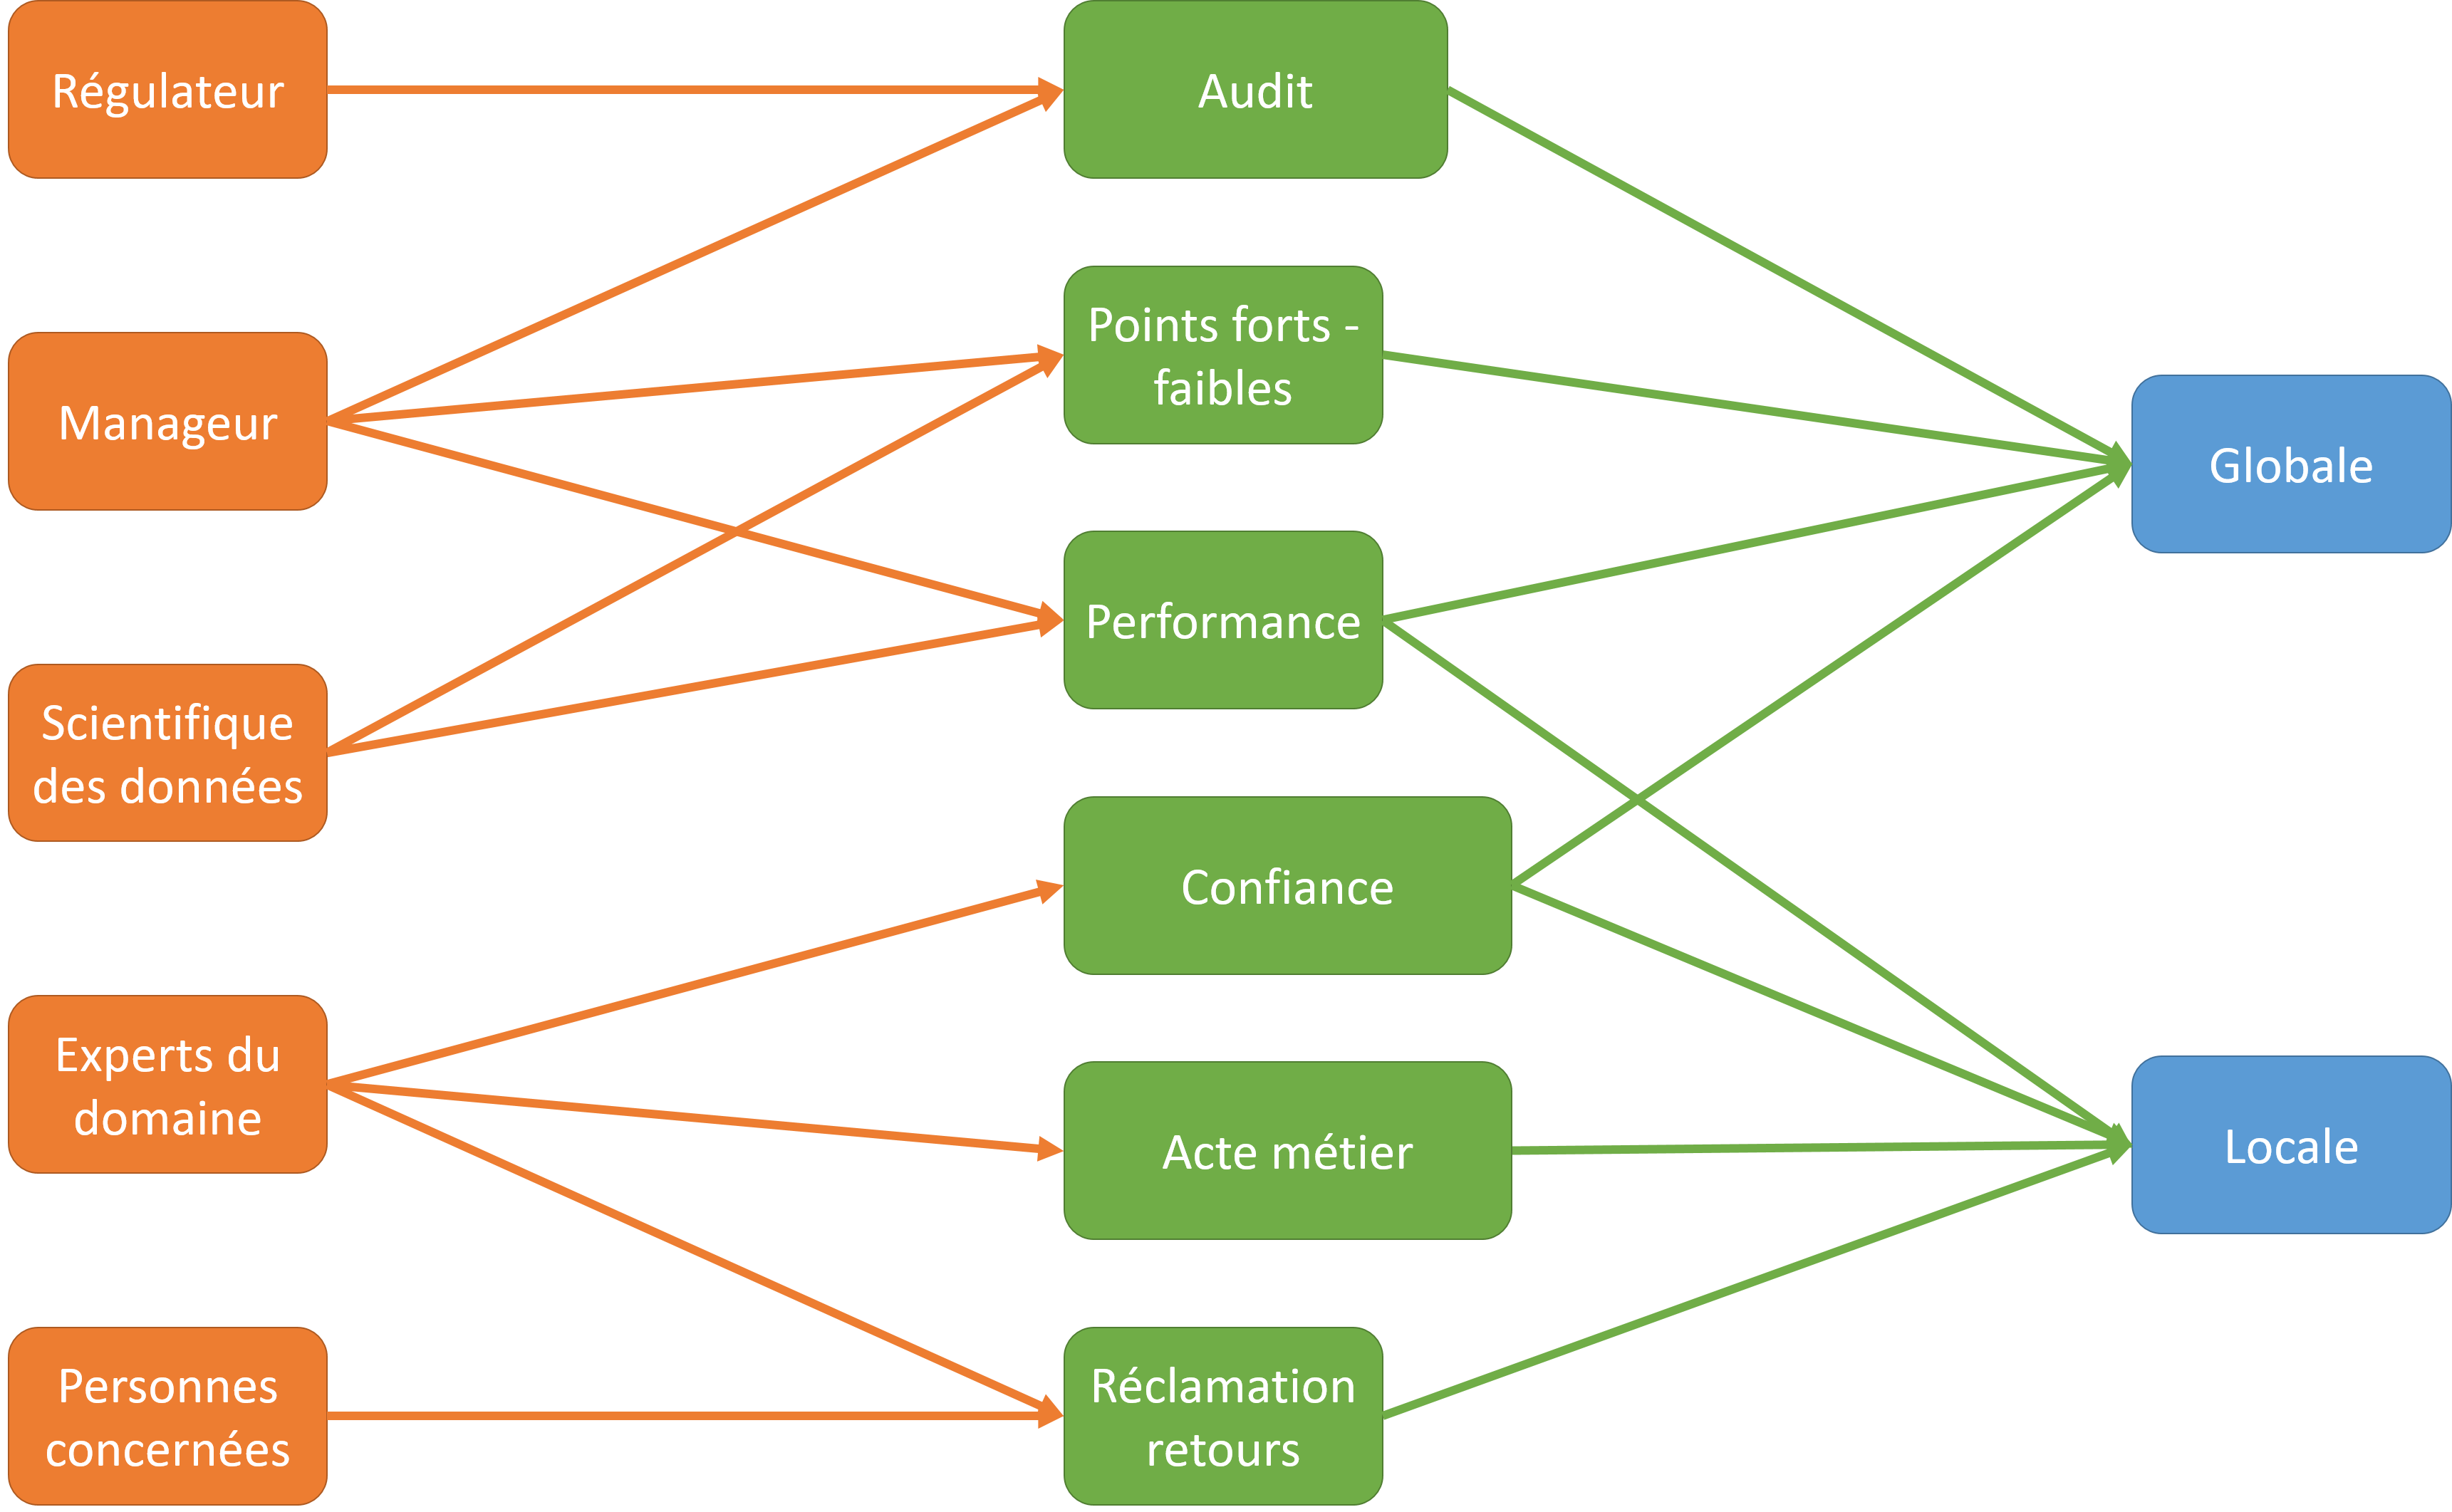
\includegraphics[scale=0.22]{S5-Presentation_du_template_nlp/figures/guide_portee.png}
    \caption{Illustration du choix de la portée selon l'utilisateur et l'objectif de ce dernier}% TODO  traduction
    \label{fig:guide_portee}
\end{figure}

% analyse guide
La figure~\ref{fig:guide_portee} montre les publics concernés, à savoir :
\begin{itemize}
    \item les régulateurs, qui s'assurent de la conformité des outils au regard de la loi,
    \item les gestionnaires du projet, qui s'assurent de l'efficacité du service rendu,
    \item les scientifiques des données, qui produisent les modèles,
    \item les experts du domaine, qui utilisent les outils ou assistent les personnes concernées,
    \item les personnes concernées par l'usage de l'outil, si celui-ci impacte leur vie.
\end{itemize}
Ces publics sont rattachés à leurs objectifs dans le cycle de vie d'un projet. Selon les organisations, les publics et objectifs peuvent varier, la figure~\ref{fig:guide_portee} sert de modélisation globale et doit être adaptée.

%exemple - détails - adaptation
Ainsi, dans la figure~\ref{fig:guide_portee}, un expert du domaine avec pour objectif de créer de la confiance dans un outil d'IA peut recevoir des explications globales ou locales. Les explications globales seront plutôt adaptées en phase de test et appropriation de l'outil, en amont de la mise en production. Les explications locales seront plus adaptées lors d'une utilisation en conditions réelles d'utilisation.

\paragraph{Choix de la stratégie}
% TODO Harold Peut-être citer un ou deux exemples de chaque type pour mieux comprendre les différentes familles ?
%facteurs dominants
La stratégie à adopter est déterminée par plusieurs facteurs tels que l'accès au système d'intelligence artificielle, sa phase de conception, et son architecture si elle est déjà choisie.
% rappel options
Les approches boites transparentes sont les plus contraignantes et les plus coûteuses à la conception, mais peuvent limiter les calculs de génération des explications à posteriori, et sont par nature fidèles au fonctionnement interne du modèle à expliquer.
Les approches boites grises sont également basées sur le fonctionnement du modèle, mais nécessitent des calculs à postériori et sont basées sur les architectures des modèles à expliquer. Elles nécessitent d'y avoir accès afin de générer l'explication.
Les approches boites noires sont les moins contraignantes, mais peuvent s'avérer coûteuses en calcul pour générer l'explication. Puisqu'il n'y a pas besoin d'avoir accès au modèle, elles sont également moins fidèles au fonctionnement interne du modèle que les autres stratégies.

% TODO Harold : figure utile ?
\begin{figure}[htpb!]
    \centering
    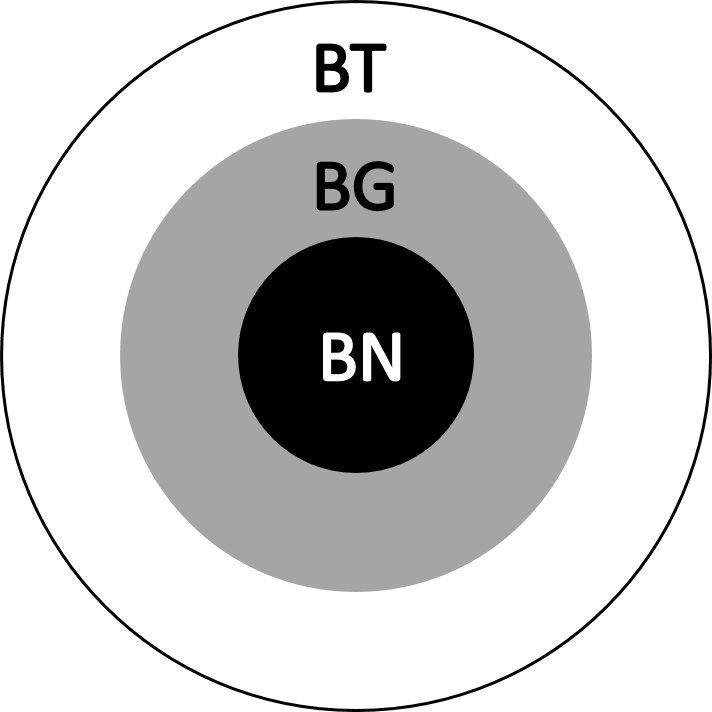
\includegraphics[scale=0.22]{S5-Presentation_du_template_nlp/figures/guide_strat2.png}
    \caption{Cercle des possibles des stratégies de la moins contraignante à la plus contraignante, du centre vers l'extérieur.}
    \label{fig:guide_strat2}
\end{figure}

La figure~\ref{fig:guide_strat2} illustre les stratégies à disposition. Au centre du cercle les stratégies boites noires (BN), sont applicables en toutes circonstances.
Lorsque les conditions sont réunies, les stratégies boites grises (BG) s'ajoutent au panel des méthodes applicables, l'étendue des méthodes à disposition est alors élargie.
Sur le même principe, les stratégies boites transparentes (BT) sont applicables sous certaines contraintes. Elles s'ajoutent alors aux autres méthodes, élargissant encore le cercle des possibles, comme l'illustre la figure\ref{fig:guide_strat2}.

\begin{figure}[htpb!]
    \centering
    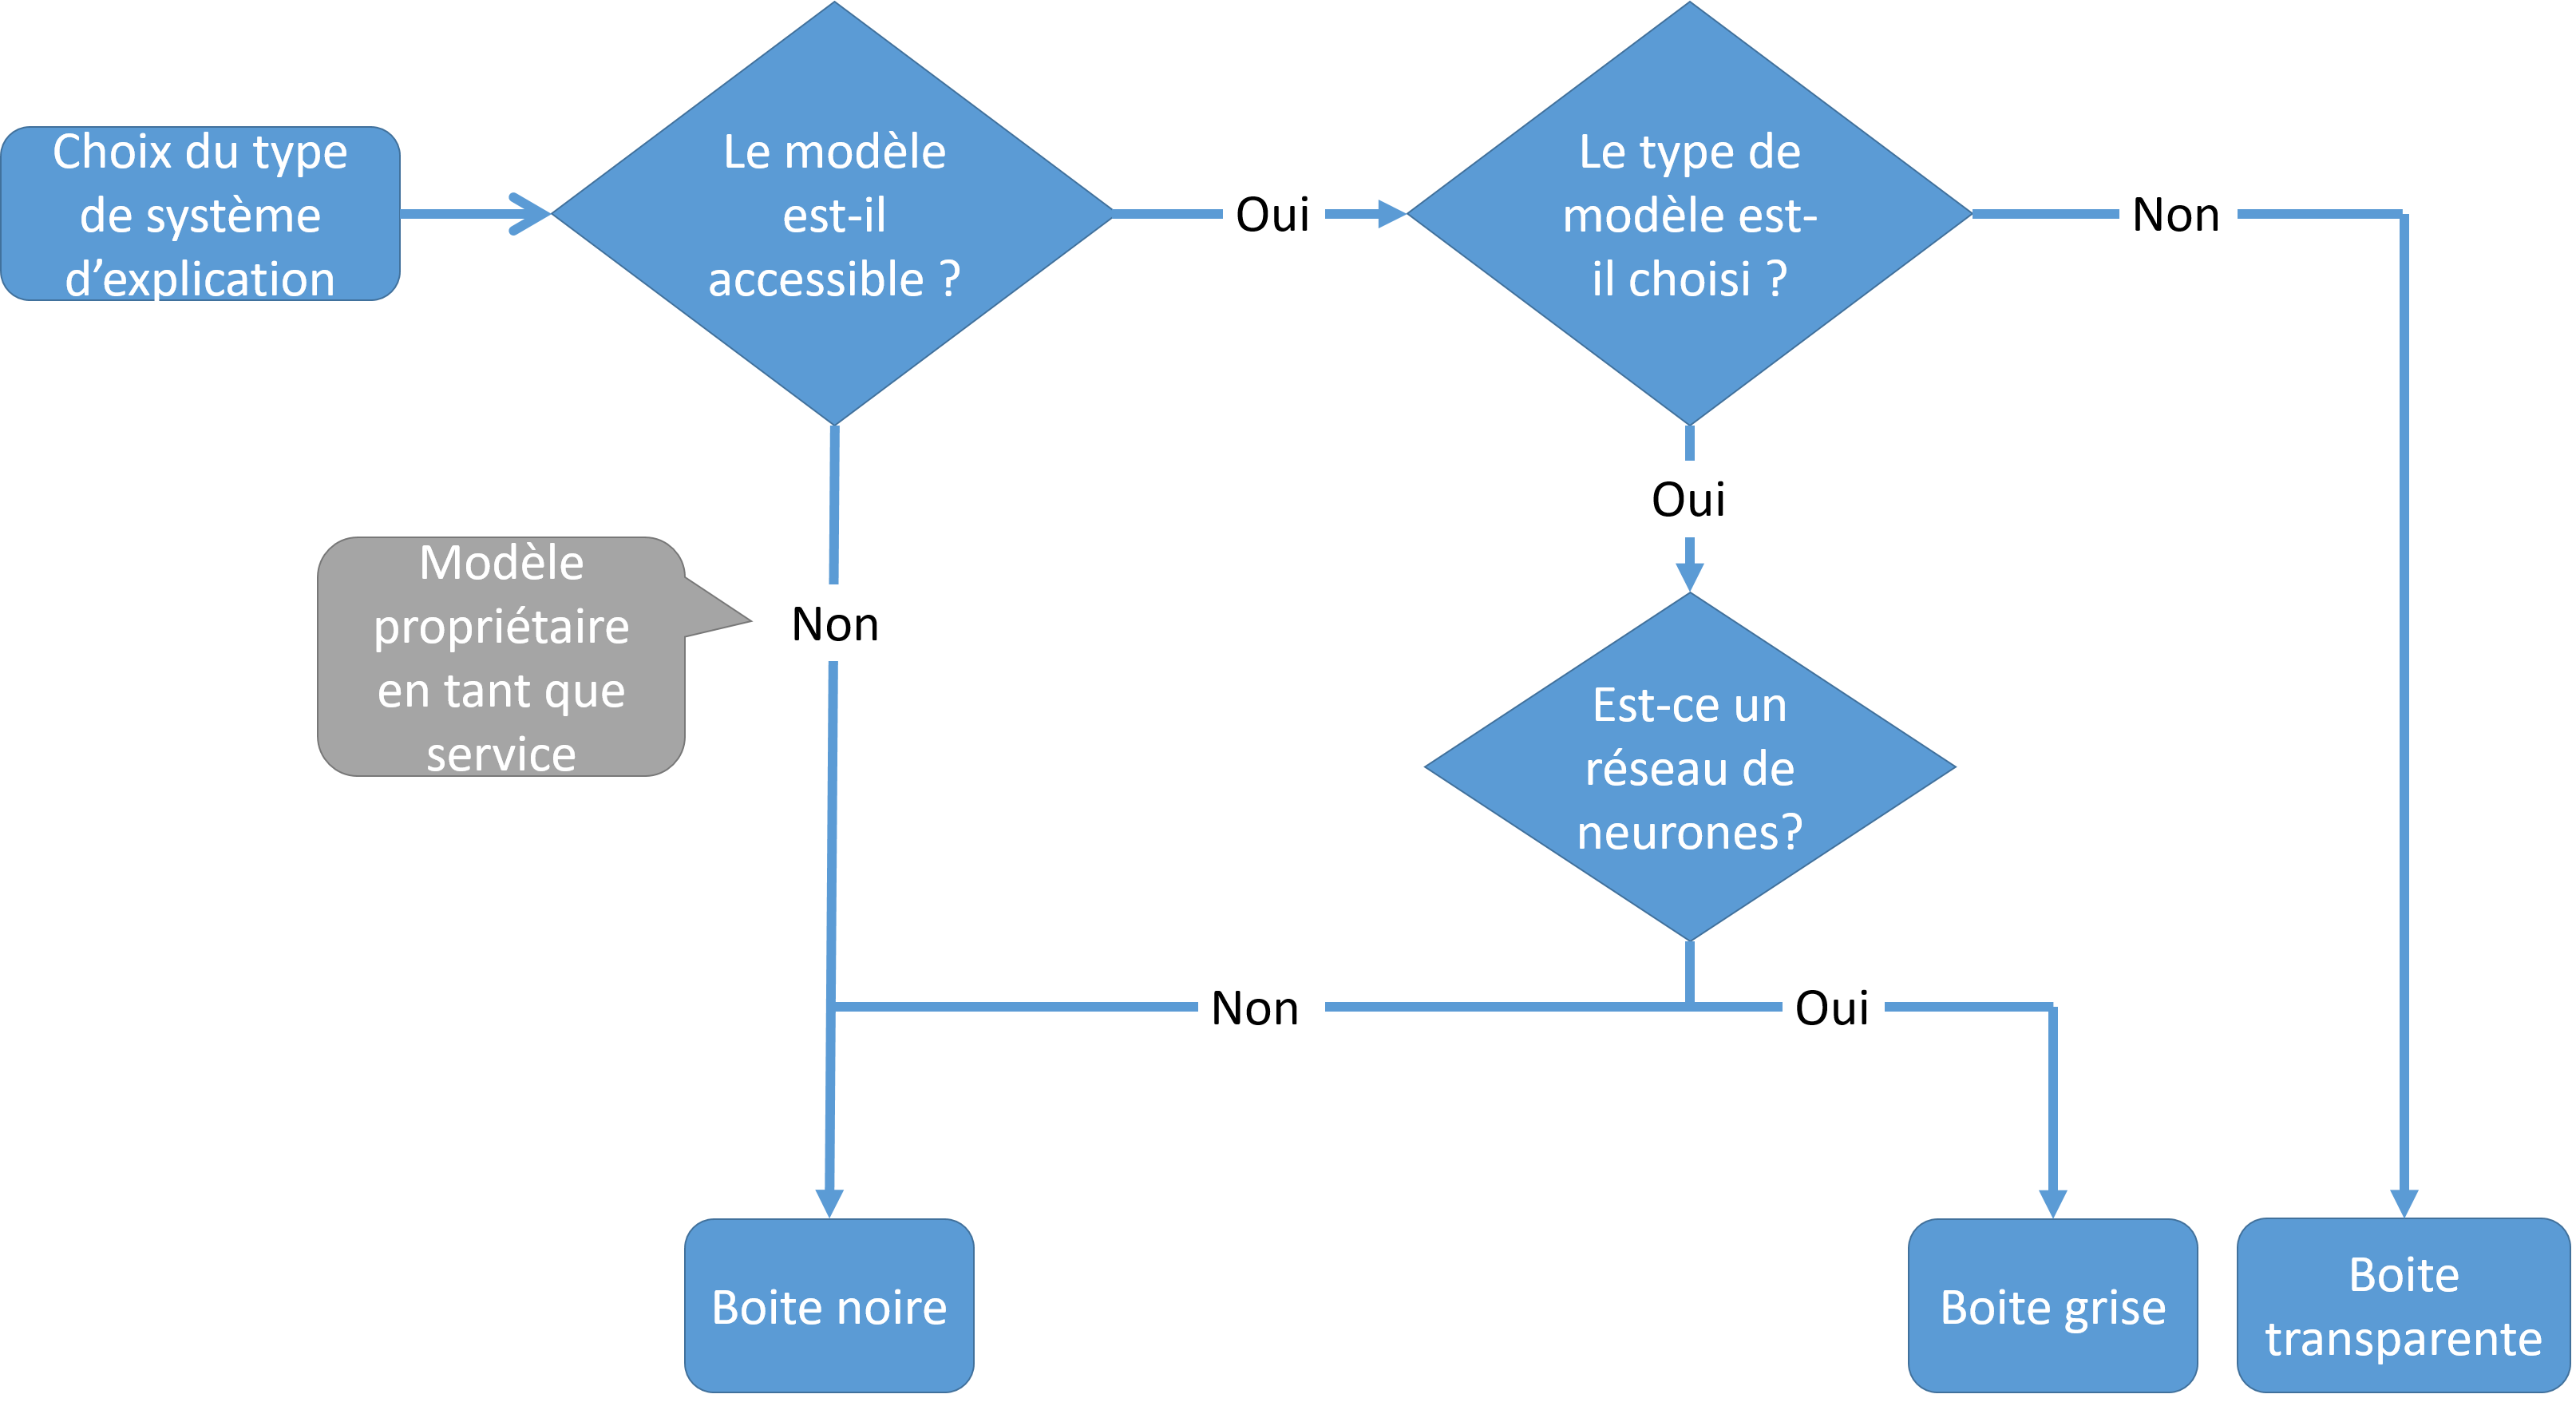
\includegraphics[scale=0.22]{S5-Presentation_du_template_nlp/figures/guide_strat.png}
    \caption{Illustration du choix de la stratégie la plus transparente applicable selon les contraintes du projet.}
    \label{fig:guide_strat}
\end{figure}

% analyse guide
La figure~\ref{fig:guide_strat} présente les choix de stratégies possibles selon les contraintes du modèle.
Le choix le moins restrictif est celui de la boite noire, applicable dans tous les cas, car il se base sur les entrées et sorties du modèle. Il est notamment adapté si le modèle est développé en externe ou si son fonctionnement interne est inaccessible pour une raison ou une autre.
Si le modèle est accessible et déjà conçu ou si son architecture est déjà choisie, alors, en fonction de cette dernière, certaines méthodes en stratégie boite grise sont applicables. Sinon, il faut se reporter sur les méthodes boites noires.
Si le modèle reste à concevoir, il est possible de concevoir son architecture avec une approche boite transparente. Les approches boite grise et boite noire restent également une option.


\paragraph{Choix du format}

Afin de choisir un type de format où un autre, il faut étudier les données à disposition et cibler les besoins des utilisateurs. La figure~\ref{fig:guide_format} schématise le choix d'un format par rapport à un autre. Si le schéma permet de privilégier une solution ou une autre, le format des explications doit s'intégrer à l'interface de l'outil où elles apparaissent. La mise en avant de variables ou d'exemples s'appuie sur des éléments concrets. Ces méthodes conviennent à une utilisation en condition réelle.
Mettre en avant une partie du contenu particulièrement utile lorsque l'exemple entier est trop long à analyser (image, texte composé de plusieurs phrases).
Les règles sont plus facilement généralisables, et sont ainsi adaptées aux audits. Les explications générées contiennent des formats plus variés, et sont à envisager lorsque les informations souhaitées ne sont pas lisibles dans les données directement : génération d'une phrase d'explications, instances menant en erreur, extraction de motifs représentatifs etc.
Si le schéma permet de privilégier une solution ou une autre, le format des explications doit s'intégrer à l'interface de l'outil où elles apparaissent.
Le test d'utilisabilité tel que présenté en section~\ref{C3:test_u} est idéalement à réaliser en complément.

\begin{figure}[htpb!]
    \centering
    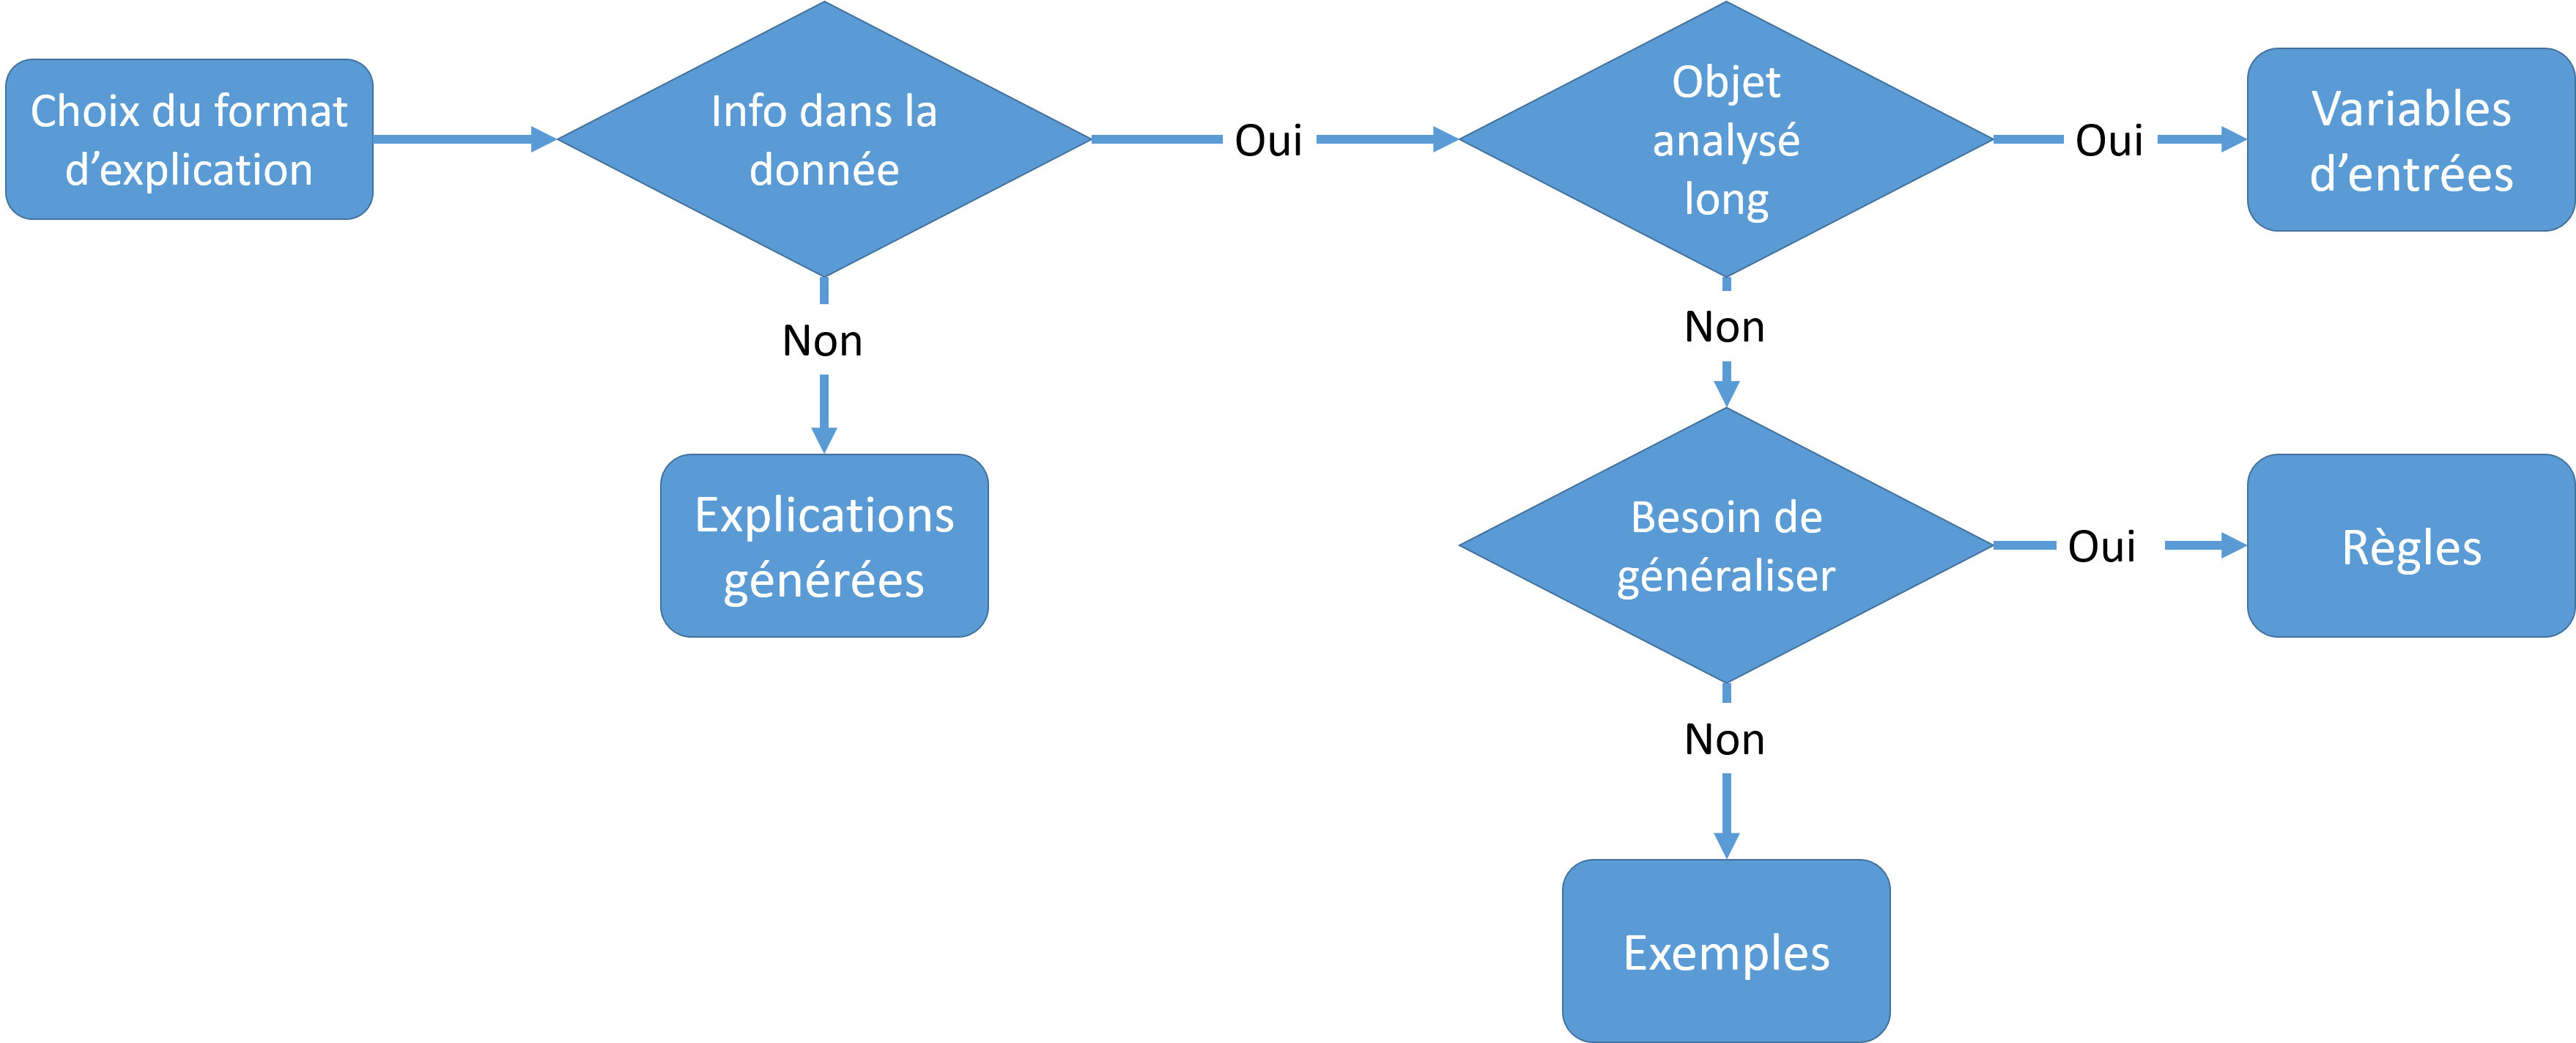
\includegraphics[scale=0.22]{S5-Presentation_du_template_nlp/figures/guide_format.png}
    \caption{Illustration du choix de format des explications selon les contraintes du projet.}
    \label{fig:guide_format}
\end{figure}

Une fois un ensemble de caractéristiques choisi, il est possible de se référer aux nombreuses méthodes de la littérature pour trouver un ensemble de méthodes d'explication candidates à  essayer.


% \subsection{Guide des méthodes de la littérature}
%
% La littérature est fournie. Le tableau~\ref{tab:eda_caracteristiques} reprend les éléments mentionnés ci-avant, en y associant les caractéristiques vues en section~\ref{C1:typologie}.
%
% \begin{table}[htpb!]
%     \caption{TODO - \textit{Format à valider} - Récapitulatif des méthodes de l'état de l'art et leurs caractéristiques associées.} \label{tab:eda_caracteristiques}
%     \begin{tabular}{|l|l|l|l|l|l|}
%         \hline
%         \textbf{Méthode}  & \textbf{Référence} & \textbf{Portée}& \textbf{Format} & \textbf{Stratégie}   & \textbf{Données} \\ \hline
%         Cartes de modèles &~\cite{Mitchell2019} & Globale & Générée & Boite grise & Toutes  \\ \hline
%         Ancres          &~\cite{Ribeiro2018}    & Locale  &  Règle  & Boite noire &  Toutes \\ \hline
%                           % &              &         &         &             &         \\ \hline
%                           % &              &         &         &             &         \\ \hline
%     \end{tabular}
% \end{table}


\section{Conclusion}
% Objectif  du chapitre
Dans ce chapitre, nous avons montré les liens entre les travaux menés et les contraintes et objectifs industriels de Pôle emploi.

% rappel Plan
Nous avons présenté l'intégration technique des travaux de thèse aux contraintes de mise en production, via l'outil \textit{Gabarit}. Nous avons également mis en avant le lien entre explicabilité et respect de la charte éthique. Finalement, nous avons donné des indications permettant aux gestionnaires de projet de sélectionner des méthodes d'explicabilité en fonction de leurs objectifs.

\boitemagique{Résumé}{
\begin{itemize}
    \item[\checkmark] Les fonctionnalités d’explicabilité sont intégrées et disponibles dans le cadre logiciel open source \textit{Gabarit}
    \item[\checkmark] L'outil \textit{Gabarit} permet de diffuser les avancées sur l'explicabilité de l'IA
    \item[\checkmark] L'explicabilité fait partie des engagements éthiques pris par l'entreprise
    \item[\checkmark] Les travaux de cette thèse permettent de répondre en partie aux engagements pris
    % \item[\checkmark]
\end{itemize}
}
